\documentclass[10pt,aspectratio=169]{beamer}

% to create handouts comment above \document and uncomment the next 3 lines
% \documentclass[10pt, handout, aspectratio=169]{beamer}
% \usepackage{styles/handoutWithNotes} % requires handoutWithNotes.sty
% \pgfpagesuselayout{4 on 1 with notes}[a4paper,border shrink=5mm]

% packages
\usepackage{graphicx}
\usepackage{multicol}
\usepackage{url}

% presentation settings
% custom theme modified from http://www.math.ucdenver.edu/~hbouwmee/resources.php
% must have beamerthemeCU.sty and cu_logo.eps in styles directory
\usepackage{styles/beamerthemeCU}
\setbeamertemplate{section in toc}[sections numbered]
% \setbeamertemplate{caption}{\raggedright\insertcaption\par} % don't display Figure for each fig
\setbeamertemplate{caption}[numbered]

% image path
\graphicspath{ {images/} }

% bibliography settings
\setbeamertemplate{bibliography item}{}	%remove the icon
%remove line breaks
\setbeamertemplate{bibliography entry title}{}
\setbeamertemplate{bibliography entry location}{}
\setbeamertemplate{bibliography entry note}{}

% presentation information
\title{PlanetiQ Pyxis: Kalman Filter}
\institute{University of Colorado Boulder}
\author{Rane Brown}
\date{\today}

% start of presentation
\begin{document}

\begin{frame}[t,plain] % t = top align, plain = no header or footer
    \titlepage
\end{frame}

\begin{frame}[t]{Table of Contents}
	\begin{center}
		\vspace{-2em}
		{\Large \textbf{\underline{Outline}}}
		\vspace{1em}
	\end{center}
	\begin{multicols}{2}
		\tableofcontents
	\end{multicols}
\end{frame} 

\section{Objectives}%-------------------------------------------------------------------------------

	\begin{frame}{Independent Study Objectives}
		\begin{itemize}
			\item Basic understanding of the Pyxis project and the importance of the Kalman filter
			\item Create unit tests for all crucial functions used by the Kalman filter
			\item Integrate C port of navigation filter into Pyxis code framework
			\item Analysis of various matrix libraries with pros and cons of each
			\item Debugging of Kalman filter upon integration into overall system
			\item Testing, tuning, and profiling of Kalman filter
		\end{itemize}
	\end{frame}

\section{Big Picture}%------------------------------------------------------------------------------

\subsection{Pyxis}
	\begin{frame}{Purpose of Pyxis Project}
	\color{red}{ADD GOOD DESCRIPTION}\\
	large scale software project
	\end{frame}

\subsection{Kalman Filter}
	\begin{frame}{What is a Kalman Filter?}
		\begin{block}{Definition}
			\begin{itemize}
				\item A set of equations that uses a recursive formula to estimate the state of a process
				\item The goal of the filter is to minimize the mean of the squared error
				\item Process and measurement noise are taken into account in order to predict the past, present, or future state of the system \cite{welch:1995}
			\end{itemize}
		\end{block}
		\vspace{.5em}
		A Kalman filter is implemented in software for the Pyxis project to help predict the location of GPS satellites in orbit.
	\end{frame}

\subsection{Coordinate Frames}
	\begin{frame}{ECEF and ECI}
		\begin{columns}
			\begin{column}{0.6\textwidth}
        \begin{block}{Earth-centered, Earth-fixed}
          A $(X,Y,Z)$ coordinate system where the point $(0,0,0)$ is defined as the center of mass of the Earth. The axes are also aligned in a fixed position with respect to the Earth's surface i.e. the earth does not rotate about an axis\cite{leick:2004}
        \end{block}
        \begin{block}{Earth-centered inertial}
          A coordinate system with the center defined as the center of mass of the Earth. The $(X,Y,Z)$ axes are fixed in place and the Earth rotates around the $Z$ axis unlike ECEF coordinates.\cite{Ashby:2004}
        \end{block}
			\end{column}
			\begin{column}{0.4\textwidth}
    			\begin{figure}
            \centering
     				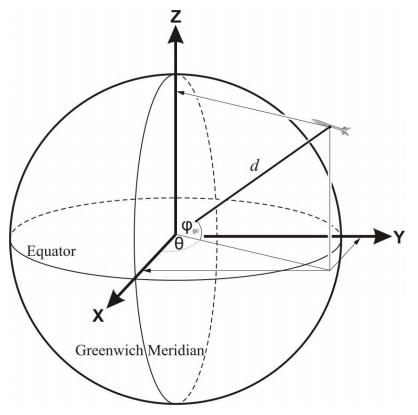
\includegraphics[width=0.3\textwidth]{ECEF}
            \caption{ECEF Coordinates\cite{polecats:2016}}
     			\end{figure}
          \begin{figure}
            \centering
            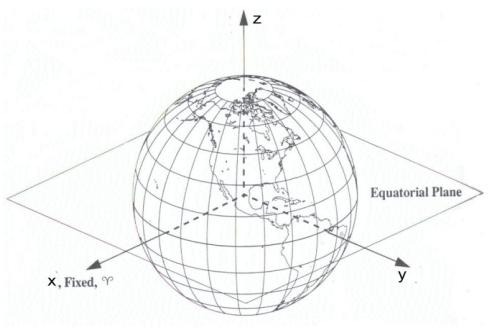
\includegraphics[width=0.4\textwidth]{ECI}
            \caption{ECI Coordinates\cite{polecats:2016}}
          \end{figure}
			\end{column}
		\end{columns}
	\end{frame}

\section{Code}%-------------------------------------------------------------------------------------

\subsection{Approach}
	\begin{frame}{Approach}
		\begin{itemize}
			\item incremental code and test
			\item use previous C port of nav filter as base
			\item different structs inputs/outputs from prev. version
		\end{itemize}
	\end{frame}

\subsection{Check Framework}
	\begin{frame}{Unit Tests}
	\end{frame}

\subsection{Git}
	\begin{frame}{Importance of Git}
	\end{frame}

\subsection{Compatibility}
	\begin{frame}{Compatibility between C and Matlab}
		reading in files
	\end{frame}

\subsection{Matrix Libraries}
	\begin{frame}{Linear Algebra}
	\end{frame}

\subsection{Testing}
	\begin{frame}{Testing and Debugging}
	\end{frame}

\subsection{Status}
	\begin{frame}{Future Work}
	\end{frame}

\section{Conclusion}%--------------------------------------------------------------------------
	\begin{frame}{Lessons Learned}
	\end{frame}

\section{References}%-------------------------------------------------------------------------------

	\begin{frame}[t]{References}
			\footnotesize
			\bibliographystyle{ieeetr} % must come before bib filename
			\bibliography{bibliography/kal_ref} 
	\end{frame}

\end{document}